\documentclass{beamer}
\usetheme{default}
\setbeamertemplate{navigation symbols}{}
%	
\usepackage{subfig}
\usepackage{epstopdf}
\usepackage{amsmath, amsthm, amssymb}
\usepackage{float}
\usepackage{rotating}
\usepackage{graphicx}
\usepackage{longtable}
\usepackage{xcolor}
\usepackage{bm}
\usepackage{tikz}
\usetikzlibrary{shapes}
\tikzset{My Arrow Style/.style={single arrow, fill=red!50, anchor=base, align=center,text width=.5cm,rotate =270}}
\newcommand{\MyArrow}[2][]{\tikz[baseline] \node [My Arrow Style,#1] {#2};}
\tikzset{My 2Arrow Style/.style={single arrow, fill=red!50, anchor=base, align=center,text width=.5cm,rotate =90}}
\newcommand{\MyArrowUp}[2][]{\tikz[baseline] \node [My 2Arrow Style,#1] {#2};}
\newcommand{\EE}{\mathbb E}
\newcommand{\var}{\mathrm{var}}
\newcommand{\cov}{\mathrm{cov}}
\newtheorem{acknowledgement}[theorem]{Acknowledgement}
\newtheorem{algorithm}[theorem]{Algorithm}
\newtheorem{assumption}{Assumption}
\newtheorem{axiom}{Axiom}
\newtheorem{case}[theorem]{Case}
\newtheorem{claim}[theorem]{Claim}
\newtheorem{conclusion}[theorem]{Conclusion}
\newtheorem{condition}[theorem]{Condition}
\newtheorem{conjecture}{Conjecture}
\newtheorem{criterion}[theorem]{Criterion}
\newtheorem{proposition}{Proposition}
\newtheorem{summary}[theorem]{Summary}
\newtheorem{exercise}{Exercise}
\newtheorem{notation}{Notation}
\newtheorem{remark}{Remark}
%\graphicspath{{graphs//}}

\title {Taxes, Debts,  and Redistributions}
\author{Anmol Bhandari, David Evans, Mikhail Golosov, Thomas J. Sargent}

\date{September 2013}
% \today will show current date.
% Alternatively, you can specify a date.
%
\begin{document}
%
\begin{frame}
\titlepage

\end{frame}


\begin{frame}
\frametitle{3 Questions}

\begin{enumerate}
 \item How costly are government debts?
 \vspace{2mm} 
 \item How do concerns for redistribution affect tax smoothing motives?
\vspace{2mm} 
 \item How should tax, transfer, debt policies respond to aggregate shocks that might also change inequality?
\end{enumerate}

\end{frame}


\begin{frame}
\frametitle{Representative agent models (I)}
Representative agent models

\begin{itemize}
\item Higher levels of debt are ``more'' distortionary. 
 \vspace{2mm} 
 \item LS: With complete markets tax rates should be smooth.  
 \vspace{2mm} 
 \item Werning: Extends the LS insights to heterogeneous agents by establishing an aggregation result.
 \vspace{2mm} 
 \item AMSS: With a risk free bond tax rates are eventually smooth and all aggregate shocks are financed using transfers.
\end{itemize}



\end{frame}

\begin{frame}
\frametitle{Representative agent models (II)}
\begin{itemize}
\item Redistribution is implicitly modeled as a non-negativity constraint on lump sum transfers. 

\vspace{2mm} 
 \item Hardwires a discontinuity in the costs of fluctuating transfers around zero.
 \begin{enumerate}
  
 \item The Ramsey planner either uses state-contingent securities to hedge aggregate shocks. 
 
 \begin{center}or \end{center}
 
 \item Accumulates a war chest of assets big enough to finance expenditures using returns on assets plus only positive transfers.
 
 \end{enumerate}

 
\end{itemize}

\vspace{2mm} 
\emph{\color{red}We begin with explicit redistribution motives  and let the government set transfers optimally. }

%   \item Representative agent models impose restrictions on transfers
%   \begin{itemize}
%  \item These are motivated only implicitly by concerns about  redistribution:  poor people can't afford lump sum taxes
%   \item These constraints \emph{almost} always bind (e.g.,  Lucas Stokey, AMSS) and drive long run debt dynamics
%   \end{itemize}
% \item We begin with explicit redistribution motives  and let the government set transfers optimally
%  \end{itemize}
% 
%  \vspace{4mm}
%  \color{red}\emph{Prescriptions for optimal tax-transfers differ substantially with explicitly modeled redistribution concerns}
%  \end{frame}
% 
\end{frame}


\begin{frame}
\frametitle{Key ingredients}


\begin{itemize}
\vspace{3mm}
 \item \textbf{Heterogeneity:} Agents are heterogeneous in 

 \vspace{2mm}
 a) Productivities 
 
 b) Pareto weights, and  
 
 c) Assets. 
 \vspace{3mm}
 \item \textbf{Instruments:} Affine tax system 
 \vspace{3mm}
 \item \textbf{Markets:} All agents trade a \emph{single} security whose payoffs can depend on aggregate shocks
\end{itemize}


\end{frame}

\begin{frame}
 \frametitle{Answers to the 3 questions}
 
\begin{enumerate}
\item \textbf{Invariance of  debt level:} 

Absent borrowing constraints, Ricardian equivalence holds. Borrowing constraints only increase welfare

\item \textbf{Invariant distribution of tax rates:} 

\begin{itemize}
	\item Has wide support
       \item The mean and variance of tax rates are driven by market incompleteness. The two ``covariances'' that matter are 
       \begin{itemize}
        \item [+]  Between returns on the asset and aggregate shocks (Public sector)
        \item [+]  Between consumption and (pre-tax) labor earnings (Private sector)
       \end{itemize}
\end{itemize}



\item \textbf{Business cycle dynamics:} (Preliminary) 
Recessions that are accompanied by higher inequality call for increase in both taxes and transfers
\end{enumerate}



\end{frame}



\begin{frame}
 \frametitle{Environment}
 \begin{itemize}
 \item \textbf{Uncertainty}: Markov aggregate shocks $s_t$
  \item \textbf{Demography}: Continuum of infinitely lived agents plus a benevolent planner
  \item \textbf{Technology}: Output $\int \theta_{i,t} l_{i,t}di$ is linear in labor supplies.
  \item \textbf{Preferences }(Households)
  \begin{equation*}
\mathbb{E}_{0}\sum_{t=0}^{\infty } \beta^t U^{i}\left(
c_{i,t},l_{i,t}\right)  \label{utility lifetime}
\end{equation*}%
\item \textbf{Preferences} (Planner): Given Pareto weights $\{\omega_i\}$
\begin{equation*}
\mathbb{E}_{0}\int \omega_i\sum_{t=0}^{\infty }\beta^t U_{t}^{i}\left( c_{i,t},l_{i,t}\right)di  \label{govmt objective}
\end{equation*}
  \item \textbf{Asset markets}: A ``risky'' bond with payoffs $\mathbb{P}=P(s|s\_)$
  \end{itemize}

\end{frame}



\begin{frame}
 \frametitle{Environment, II}
 \begin{itemize}
  \item \textbf{Affine Taxes}: Agent $i$'s tax bill
\[- T_t + \tau_t \theta_{i,t}l_{i,t}\]

\item[]
  \item \textbf{Budget constraints} Let $R_{t-1,t}=\frac{P_t}{q_{t-1}}$
  \begin{itemize}
   \item Agent $i$: $ c_{i,t}+b_{i,t}=\left( 1-\tau _{t}\right) \theta _{i,t}l_{i,t}+R_{t-1,t}b_{i,t-1}+T_{t}$
\item Government: $g_{t}+B_{t}+T_t=\tau _{t}\int \theta_{i,t}l_{i,t}di+R_{t-1,t}B_{t-1}$
  \end{itemize}

\item[]
  \item \textbf{Market Clearing}
  \begin{itemize}
   \item Goods: $\int c_{i,t}di+g_t =\int \theta _{i,t} l_{i,t}di$

   \item Assets: $\int b_{i,t}di +B_{t}=0$

  \end{itemize}
  \item[]

\item \textbf{Initial conditions}: Distribution of assets $(\Psi_0(b_{i,-1}),B_{-1},s_{-1})$
\end{itemize}
\end{frame}



\begin{frame}
 \frametitle{Ramsey Problem}

\begin{definition}
\textbf{Allocation, price system, government policy}: Standard

\end{definition}

\begin{definition}
\textbf{Competitive equilibrium}: Given $\left( \Psi_0(b_{i,-1})
_{i},B_{-1},s_{-1}\right) $ and $\left\{ \tau _{t},T_{t}\right\} _{t=0}^{\infty }$
all allocations are chosen optimally, markets clear \footnote{Usually, we impose only  ``natural'' debt limits. }
\end{definition}

\begin{definition}
\textbf{Optimal competitive equilibrium}: A welfare-maximizing competitive
equilibrium for a given $\left( \Psi_0(b_{i,-1}),B_{-1},s_{-1}\right) $
\end{definition}

 \end{frame}

% \begin{frame}
% \frametitle{Contrast with representative agent models}
%  Representative agent with linear taxes
% \begin{itemize}
%  \item Higher levels of debt are distortionary
%  \item With incomplete markets (as in  AMSS), the optimal  government policy is to accumulate assets
%  \end{itemize}
% 
%  \end{frame}
%
%  \begin{frame}
%  \frametitle{Does AMSS Confirm Reinhart-Rogoff Fears?}
%  \begin{itemize}
%  \item Higher govt.\ debts are more  distorting, but $\ldots$
%  \item Because it is distortionary, asymptotically govt. doesn't issue debt
%  \end{itemize}
%  Things change in our environment
%  \end{frame}

%  \begin{frame}
%  \frametitle{Redistribution and optimal transfers}
%  \begin{itemize}
%   \item Representative agent models impose restrictions on transfers
%   \begin{itemize}
%  \item These are motivated only implicitly by concerns about  redistribution:  poor people can't afford lump sum taxes
%   \item These constraints \emph{almost} always bind (e.g.,  Lucas Stokey, AMSS) and drive long run debt dynamics
%   \end{itemize}
% \item We begin with explicit redistribution motives  and let the government set transfers optimally
%  \end{itemize}
% 
%  \vspace{4mm}
%  \color{red}\emph{Prescriptions for optimal tax-transfers differ substantially with explicitly modeled redistribution concerns}
%  \end{frame}
% 
% \begin{frame}
%  \frametitle{Main working parts}
% \begin{itemize}
%  \item \textbf{Welfare Criterion}: Benevolent planner with explicit redistribution motives
%  \item \textbf{Instruments}: Transfers and a flat tax on labor income
%  \item \textbf{Restrictions}:
%  \begin{enumerate}
%   \item The tax on labor income is linear in wage earnings
%   \item Transfers are unrestricted in sign and magnitude  but not  conditioned on agents' identities
%   \item Incomplete markets
%  \end{enumerate}
% \item \textbf{Trade-offs}:
% \begin{enumerate}
% \item Varying labor taxes imposes dead weight losses
% \item With  explicit redistribution motives come costs of fluctuating transfers. Withdrawing a unit of consumption affects rich and poor people differently
% \end{enumerate}
% \end{itemize}
% \end{frame}
% \begin{frame}
%  \frametitle{Key forces }
%  \begin{itemize}
%   \item \textbf{Heterogeneity}
%   \begin{enumerate}
%   \item Two sources of heterogeneity: Productivities and asset holdings
%    \item Unrestricted transfers $\rightarrow$ \emph{Level }of government debt is irrelevant, what matters is its \emph{distribution} across agents
% 
%   E.G, productive agents holding a lot of government debt can be more distortionary
%   \end{enumerate}
%   \item \textbf{Responses}
% 
%   Since welfare costs depend on the distribution of assets, optimal policy is affected by and affects the distribution of net assets
% \begin{enumerate}
% \item \textbf{Absence of agent specific transfers}: This prompts the govt. to engineer  a negative correlation between net assets and labor earnings
% \item \textbf{Absence of state contingent securities}: This prompts the govt. to exploit endogenous fluctuations in the interest rate
% 
%  \end{enumerate}
% \end{itemize}
% 
% \end{frame}
% 
%
% \begin{frame}
% \frametitle{Key mechanisms}
% Two departures from representative agent models:
% \begin{itemize}
% \item \textbf{Unrestricted transfers}: Level of debt is not distortionary. What matters is how it is distributed across agents
%  \item \textbf{Explicit redistribution motives}: Endogenous costs of fluctuating transfers. Taking away a unit of consumption good affects ``rich'' and ``poor'' people differently
%  \end{itemize}
%
% \emph{One part of heterogeneity (productivities) is exogenous but heterogeneity in assets is endogenous. }
%
%
% \end{frame}



\begin{frame}

\frametitle{Ramsey problem: Recursive formulation}

Split  into two parts

\begin{enumerate}
\vspace{3mm}
\item $\mathbf{t\geq1}$: Ex-ante continuation problem with state variables $\{\Gamma_{t-1}(x_{i,t-1},m_{i,t-1},\theta_{i,t-1}),s_{t-1}\}$, where

\begin{itemize}
 \item Scaled assets: $x_{i,t-1}=u_{c,i,t-1}b_{i,t}$
 \item Scaled ``market weights'': $m_{i,t-1}\propto \frac{1}{u_{c,i,t-1}}$
\end{itemize}

% 
% \[\bm{x}= \beta_{t-1}^{-1}\left( U_{c,t-1}^{2}\tilde{b}_{2,t-1},...,U_{c,t-1}^{I}\tilde{b}_{I,t-1}\right)\]
% \[ \bm{\rho }=\left( U_{c,t-1}^{2}/U_{c,t-1}^{1},...,U_{c,t-1}^{I}/U_{c,t-1}^{1}\right) \]
\vspace{3mm}
\item $\mathbf{t=0} $: Ex-post initial problem with state variables $(\Psi_0(b_{i,-1}),s_{0})$
\end{enumerate}

\end{frame}

\begin{frame}
 \frametitle{Bellman Equation for  $t\geq1$}
 \scriptsize

\begin{equation*}
V(\Gamma_{\_},s\_)=\max_{\substack{c_{i}(s),l_{i}(s),x_{i}(s),m_{i}(s)\\\tau(s),T(s),\alpha_1,\alpha_2(s)} }
\sum_{s}\Pr (s|s\_)\left[ 
\int \omega_iu(c_i(s),l_i(s))di  +\beta V(\Gamma(s),s)\right]
\end{equation*}%



where the maximization is subject to
\begin{subequations}
\begin{equation*}
\label{eq-imp}
\frac{x_{i,\_}u_{i,c}(s)P(s|s\_)}  {\beta\mathbb{E}^i_{s\_}u_{i,c}(s)P(s|s\_)} = u_{i,c}(s)[c_i(s)-T(s)]+u_{i,l}(s)l_{i}(s)+x_i(s)
\end{equation*}



\begin{equation*}
\label{eq-Bond_1}
\alpha^1 =m_{i,\_}\mathbb{E}^i_{s\_}u_{i,c}(s)
\end{equation*}

\begin{equation*}
\label{eq-Bond_2}
\alpha^2(s)=m_i(s)u_{i,c}(s)
\end{equation*}

\begin{equation*}
\label{eq-wages}
-u_{i,l}(s)=[(1-\tau(s)] u_{i,c}(s) \theta_i(s)
\end{equation*}


\begin{equation*}
\label{eq-norm-m}
\int m_i(s) di=1
\end{equation*}

\begin{equation*}
\label{eq-resources}
\int l_i(s) \theta_i(s) di = \int c_i(s) di+g(s)
\end{equation*}
\end{subequations}

\end{frame}

\begin{frame}
\frametitle{Bellman equation for $t=0$}

 \begin{equation*}
V_0\left(\Psi_0(b_{i,-1}), s_0\right) = \max_{\substack{c_{i,0},l_{i,0},x_{i,0},m_{i,0}\\ \tau_0,T_0}} {\int \omega_i U^i(s_0) + \beta V\left(\Gamma_0, s_0\right)}
\end{equation*}
where the maximization is subject to
\begin{subequations}
%\textcolor{red}{XXXXX Should  a similar change to the one David recommended be executed here?}
\begin{equation*}
\label{eq-imp}
b_{i,-1}u_{i,c,0} = u_{i,c,0}[c_{i,0}-T_0]+u_{i,l,0}l_{i,0}+x_{i,0}
\end{equation*}



\begin{equation*}
\label{eq-wages}
-u_{i,l,0}=(1-\tau_0) u_{i,c,0} \theta_{i,0}
\end{equation*}


\begin{equation*}
\label{eq-norm-m}
\int m_{i,0} di=1
\end{equation*}

\begin{equation*}
\label{eq-resources}
\int l_{i,0} \theta_{i,0} di = \int c_{i,0} di+g_0
\end{equation*}
\end{subequations}


\end{frame}

\begin{frame}
 \frametitle{A review of LS and AMSS}
 \begin{itemize}
  \item Both impose $T_t\geq0$
  \item The multiplier on the implementability constraint $\mu_t$,
  \begin{itemize}
   \item LS: Constant\[\mu_t=\mu_0\]
   
   With CES preferences tax rates are smooth.
   
   \item AMSS: Positive risk adjusted martingale \[\mu_t=\mathbb{E}_tu_{c,t+1}\mu_{t+1}\]
  
  With QL preferences $\mu_t$ converges to zero and tax rates converge to zero
  
  \end{itemize}
\item This makes the constraint on transfers either always slack or eventually slack.
 \end{itemize}

\end{frame}



 \begin{frame}
  \frametitle{Ricardian Equivalence}
  \begin{itemize}
   \item \textbf{Result}: A large set of transfers and asset profiles support the same competitive allocation
   
   \emph{Taking away a unit of all agents' assets and increasing transfers by a unit leaves budget sets unchanged}
   
   \vspace{2mm}
   
   \item \textbf{Implication:} Ceteris paribus, an economy with higher level of initial government debt  but same relative holdings has the same welfare
   
   \vspace{2mm}
   
   \item \textbf{Corollary:} Exogenous borrowing constraints of the form $b_{it}>\underline{b}_i$ are not restrictive
\vspace{2mm}
   
   
 \emph {If some borrowing constraints bind, the planner can change transfers to  slacken   \emph{all}  of them}
  \end{itemize}
  \color{red}\emph{Thus, Ricardian equivalence holds with distortionary taxes and ad hoc borrowing limits}

\end{frame}



\begin{frame}
 \frametitle{Active channels}
  \begin{enumerate}
\item Varying labor taxes imposes dead weight losses.


\item Fluctuating transfers is costly because of concerns for redistribution. 

\item Effects of taxes on redistribution depends on cross sectional heterogeneity of consumption and earnings.

\item The benefits of fluctuating transfers depend of limits to fiscal hedging.

\end{enumerate}

 \end{frame}
\begin{frame}
 \frametitle{Understanding the channels}
 \begin{enumerate}
  
  \item Study a two type QL economy: This will shut down idiosyncratic risk  
  \begin{itemize}
   
   \item Costs of transfers will come from Pareto weights
   \item Hedging motive will be controlled using payoffs $P(s)$
  \end{itemize}

  \item More generally 
  \begin{itemize}
   \item Costs of transfers will come from spreads in marginal utilities. A key determinant will be the nature of idiosyncratic risk.
   \item Hedging motives will depend on covariance of asset returns with aggregate shocks
   \end{itemize}
\item Study a calibrated economy  

 \end{enumerate}

 
\end{frame}


\begin{frame}
 \frametitle{Simple Example: 2 Agent QL economy}
 Consider a ``seemingly'' AMSS economy
 \begin{enumerate}
  \item Two classes of agent with constant productivities $\theta_1=0,\theta_2>0$
  \item Preferences given by $U(c,l)=c-\frac{l^{1+\gamma}}{1+\gamma}$
  \item Pareto weights $\{\omega,1-\omega\}$
  \item Only i.i.d aggregate shocks to $g(s)$
 \end{enumerate}
 
 \textbf{Normalization:} Let the assets of the productive agent be denoted by $b$
\end{frame}


\begin{frame}
 \frametitle{Case 1: Risk free bond}
\begin{theorem}
Let $\omega>\bar{\omega}$ and  suppose $P(s)=1$, $\lim_t \tau_t=-\infty$, $\lim_t b_t=-\infty$     a.s
\end{theorem}

\vspace{3mm}

\begin{corollary} Suppose we augment our problem with a constraint $b_{t}\geq \underline{b}.$ Then with risk-free debt there is an invariant distribution $\psi .$ Morever, for any $\hat{b}\in \left( \underline{b},\bar{b}_n\right) ,$ $\psi \left( \left[ \underline{b},\hat{b}%
\right] \right) >0$ and $\psi \left( \left[ \hat{b},\bar{b}_n\right] \right)
>0.$. 
\end{corollary}


\vspace{3mm}
\emph{\color{red}The invariant distribution of taxes is wide as fluctuations in transfers are costly}

\end{frame}



\begin{frame}
 \frametitle{Case 2: Perfect hedging}
\begin{theorem}
Let $\omega>\bar{\omega}$ and suppose $\overline b < \overline b_n$ and payoffs satisfy
\[P(s) = 1- \frac{\beta}{\overline b}(g(s) - \mathbb{E} g)\] 
			 then for all $b_{-1}$, $b_t\rightarrow \overline b $ a.s 
\end{theorem}


\begin{corollary} Suppose we augment our problem with a constraint $b_{t}\geq \underline{b}<\bar{b}.$ Then the invariant distribution of $b$ (and also tax rates) is degenerate with $\bar{b}=-\beta\frac{\var[g(s)]}{\cov[P(s),g(s)]}$ 
\end{corollary}


\emph{\color{red} The limiting allocation corresponds to a complete market Ramsey problem}
\end{frame}


\begin{frame}
 \frametitle{Case 3: Imperfect hedging}

\textbf{Decompose payoffs} \[P(s)=\hat{P}(s)+\bar{P}(s)\] 

where	$\overline{P}(s) = 1- \frac{\beta}{\overline b}( g(s) - \mathbb{E} g)$ and  $\hat{P}(s)$ is orthogonal to $g(s)$. 

	

\begin{theorem}
For $\omega>\bar{\omega}$, the ergodic distribution of debt of the policy rules linearized around $(\overline b, \overline{P}(s))$ will have mean $\overline b$ and and coefficient of variation
	\[
		\frac{\sigma_b}{\overline b}\leq \sqrt\frac{\var(P(s)) - |\cov(g(s),P(s))|}{|\cov(g(s),P(s))|}
	\]

	The speed of convergence to the ergodic distribution given by
	\[
		\frac{\EE_{t-1}(b_t-\overline b)}{(b_{t-1} - \overline b)} = \frac1{1+|\cov(P(s),g(s))|}
	\]


\end{theorem}
 \end{frame}



\begin{frame}
 \frametitle{Adding risk aversion}
 
 \textbf{Modifications:}
 \begin{itemize}
  \item Endogenous component to covariance between payoffs and expenditure needs.
  
  \item Costs of transfers come from spreads in marginal utilities.
  
  
  \end{itemize}

  
 \textbf{Implications:}
  
  \begin{enumerate}
   \item Inequality distortions both call for a negative correlation between productivities and net assets. 
   \item This is exacerbated with countercyclical returns on fiscal assets

  \end{enumerate}


\end{frame}







\begin{frame}
\frametitle{ Inequality distortions}

\vspace{2mm}
\MyArrow{} TFP: Adjust tax rate $\tau$ or transfers $T$, both are costly

\vspace{2mm}
Suppose $b=0$
\begin{enumerate}
 \item Present value of earnings of productive agent are higher
 \item A reduction in transfers hurts the low productivity agent more
\end{enumerate}

Then

 \MyArrow{} $b$ is same as increasing the \textbf{debt} of the productive agent

\color{red} This drives the after-tax, after-interest incomes of both agents  closer
together



\end{frame}




% \begin{frame}
% \frametitle{ Inequality distortions}
%
% %\textcolor{blue}{Anmol XXXXX: may we please discuss this slide? It needs some clarification.}
% Start with a spread in discount factors set to equalize interest rates  across states,  i.e., $R(s_l)=R(s_h)$. Then SS  $x>0$
%
% \vspace{2mm}
% \MyArrow{} TFP ($\theta_1$): Adjust tax rate $\tau$ or transfers $T$, both are costly
%
% \vspace{2mm}
% Suppose $x=0$ or $b_{2}(s)=b_{1}(s)$,
%
% \MyArrow{} Then reductions in transfers hurt the low productivity agent more
%
% \vspace{2mm}
%
%  \emph{A fall in transfers that increases inequality gives rise to a cost  not present in  representative agent economies. This gives the planner an incentive to reduce the costs of  inequality distortions by $\ldots$ }
%
%  \MyArrowUp{} $x$
%
% \color{red} Reducing the relative asset holdings of the productive agent eventually drives the after-tax, after-interest incomes of both agents  closer
% together
%
%

%\end{frame}

\begin{frame}
\frametitle{Interest rate fluctuations}
\begin{itemize}

 \item \textbf{Countercyclical interest rates: }

 \MyArrow{} TFP: If the  tax rate  $\tau $ is left unchanged, the government faces a shortfall of revenues.

 \begin{enumerate}
 \item Reminder: $b$ is \textbf{debt} of the government
\item By holding positive assets the govt. can use higher interest income to offset some revenue losses from its tax on labor in recessions
  \item This force is present in representative agent economies with endogenous fluctuations in interest rates
\end{enumerate}

 \MyArrow{} The government reduces debt $b$ 

 \end{itemize}



\end{frame}


\begin{frame}
 \frametitle{Adding idiosyncratic risk}
 \begin{itemize}
  \item Eliminates negative correlation between pre-tax earnings and assets. 
  \vspace{3mm}
  \item Joint distribution of consumption and pre-tax earnings drives the mean level of taxes
\vspace{3mm}
  
  \item The spread of the ergodic distribution is mainly a determined by public sector's fiscal hedging abilities
 \end{itemize}

 \end{frame}
 \begin{frame}
 \frametitle{Decomposing the tax rate}
Define $w_{i,t}=u^i_{c,t}[\omega^i-\mu^i_t(1+\gamma)]$ and $\bar{w}_{t} = \int u^i_{c,t}\omega^i di$ and $\bar{w}_{i,t}=\frac{g_{i,t}}{\bar{w}_t}$.

 
\begin{equation*}
	\label{eq-labor_taxes}
\frac{1}{1-\tau_t}= \underbrace{\frac{\hat{Y}_t}{Y_t}}_{\substack{\text{Effectiveness}\\ \text{of} \\ \text{Taxes}}}   \underbrace{\frac{\bar{w}_t }{\lambda_t}}_{\substack{\text{Benefits} \\ \text{of} \\ \text{Transfers}}}
\end{equation*}   

Where $Y_t=\int y^i_t di$ and $\hat{Y}_t=\int y^i_t \bar{w}_{i,t}di$


\end{frame}



\begin{frame}
 \frametitle{Two stark cases}
\begin{enumerate}
 \item Start with a representative agent economy with no aggregate shocks. 
\item 
 Consider two process for idiosyncratic risk
 
 \begin{itemize}
  \item IID shocks
  
  \item Persistent (close to unit root) shocks
 \end{itemize}

\end{enumerate}
 

How to taxes evolve as the distribution fans out?
 
\end{frame}

\begin{frame}
\frametitle {Tax rates in the IID economy}
  \begin{figure}[htp]
 \centering
 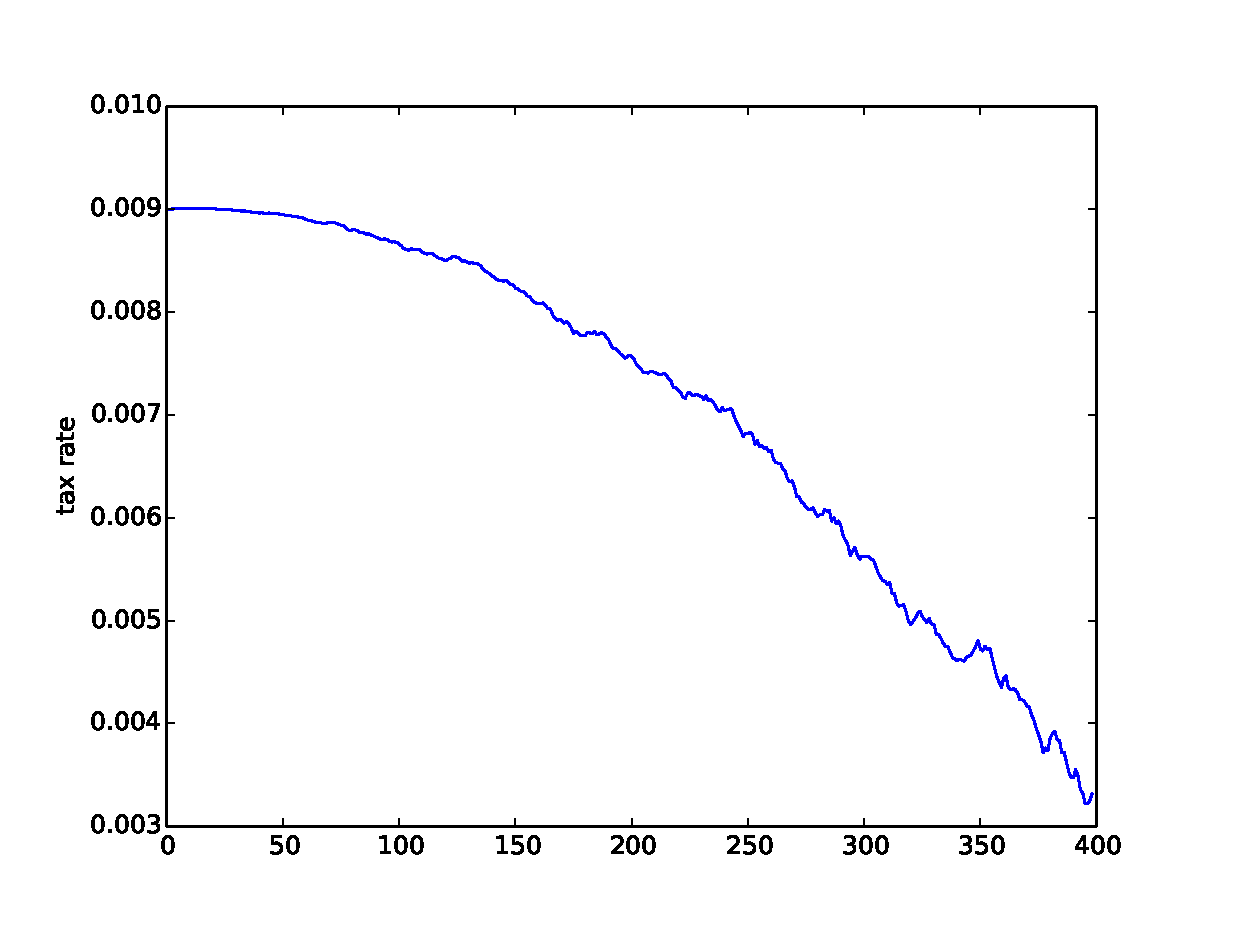
\includegraphics[width=0.9\textwidth]{Images/tax_iid.eps}
 \caption{Taxes in the iid economy.}
 \label{fig:taxes_iid}
 \end{figure}
\end{frame}

\begin{frame}
\frametitle {Tax rates in the close to unit root economy}

  \begin{figure}[htp]
 \centering
 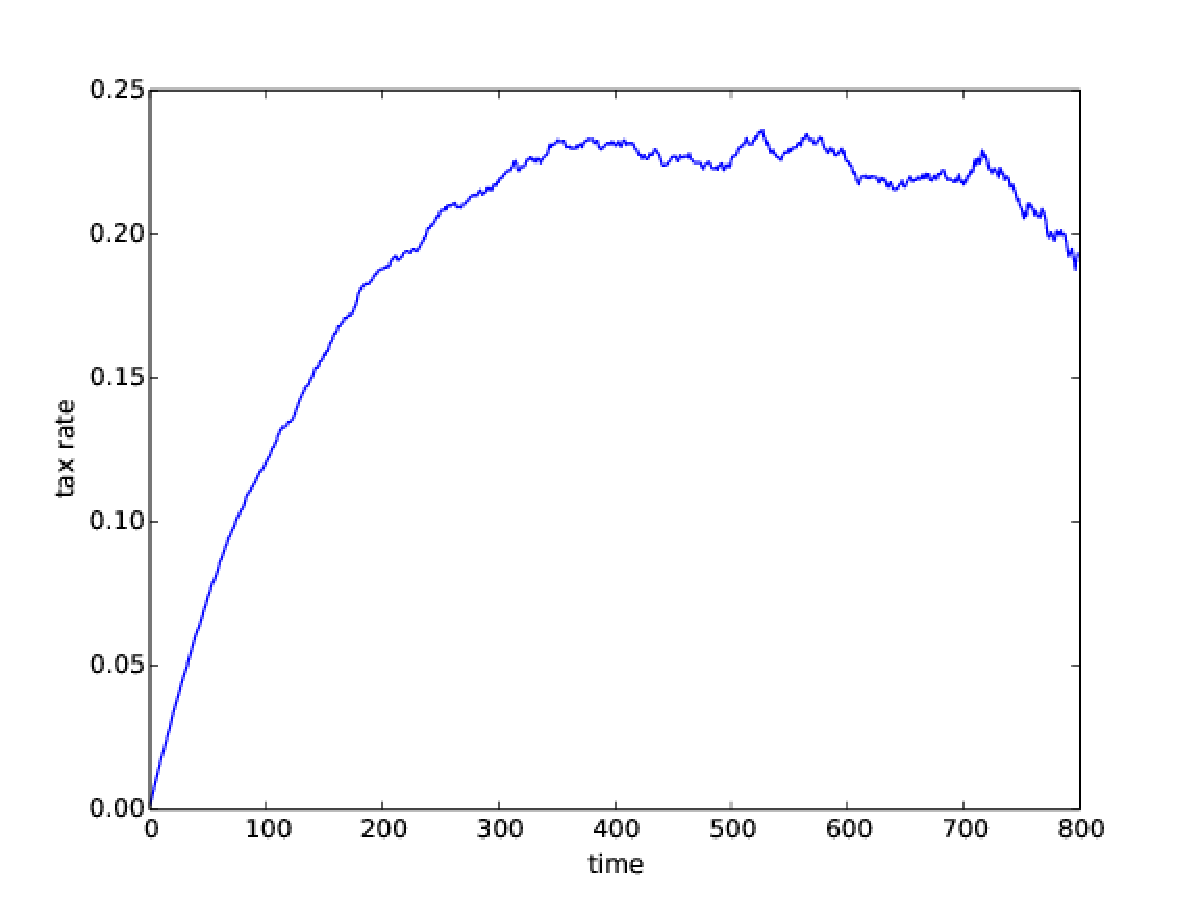
\includegraphics[width=0.9\textwidth]{Images/near_unit_tax.pdf}
 \caption{Taxes in the close to unit root economy.}
 \label{fig:taxes_pers}
 \end{figure}
\end{frame}

\begin{frame}
  \begin{figure}[htp]
 \centering
 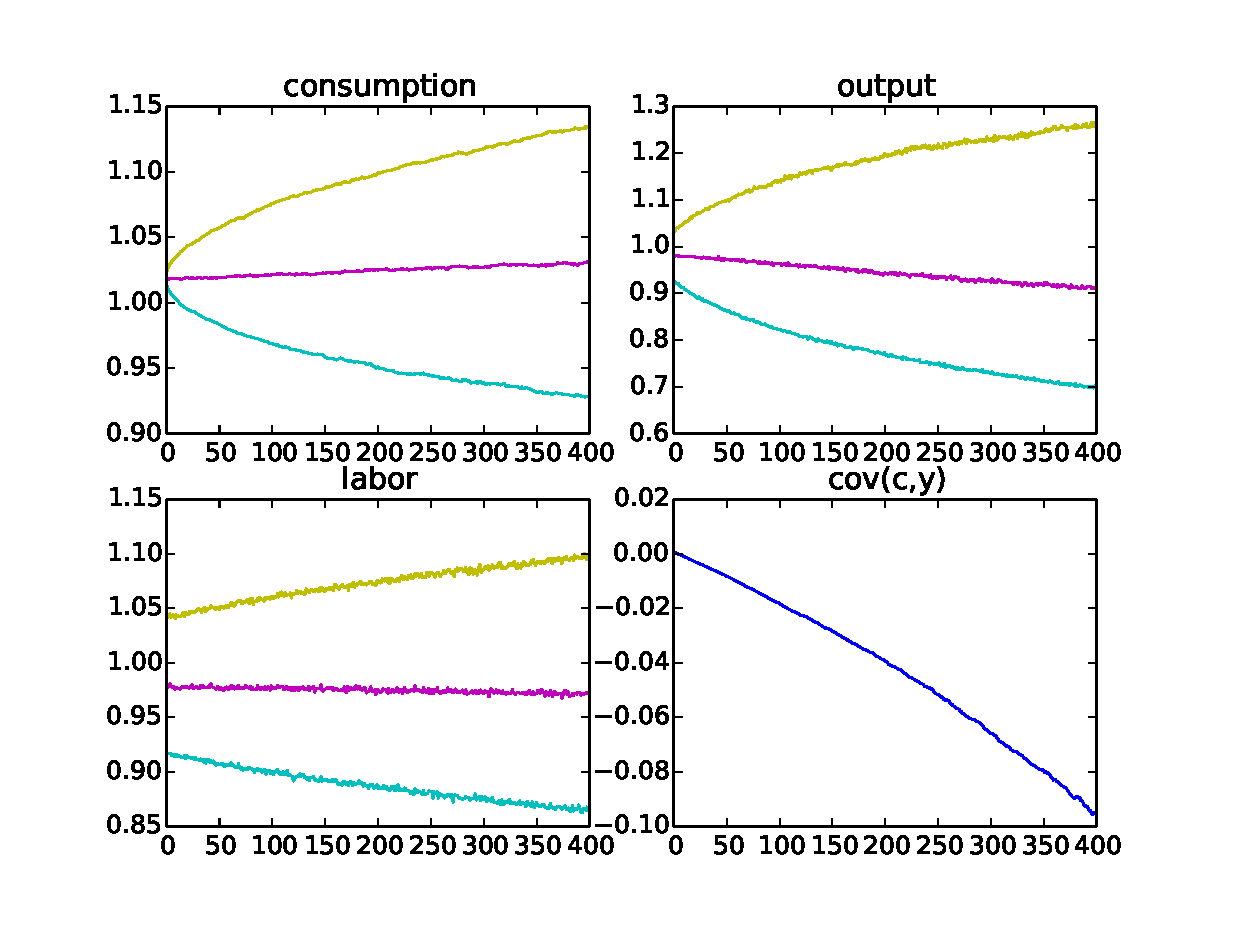
\includegraphics[width=0.8\textwidth]{Images/quant_iid.eps}
 \caption{Inequality in the iid economy. The figure plots the quantiles for consumption, pre-tax labor earnings, labor and the covariance between consumption and pre-tax labor earnings}
 \label{fig:quant_iid}
 \end{figure}
\end{frame}

\begin{frame}
  \begin{figure}[htp]
 \centering
 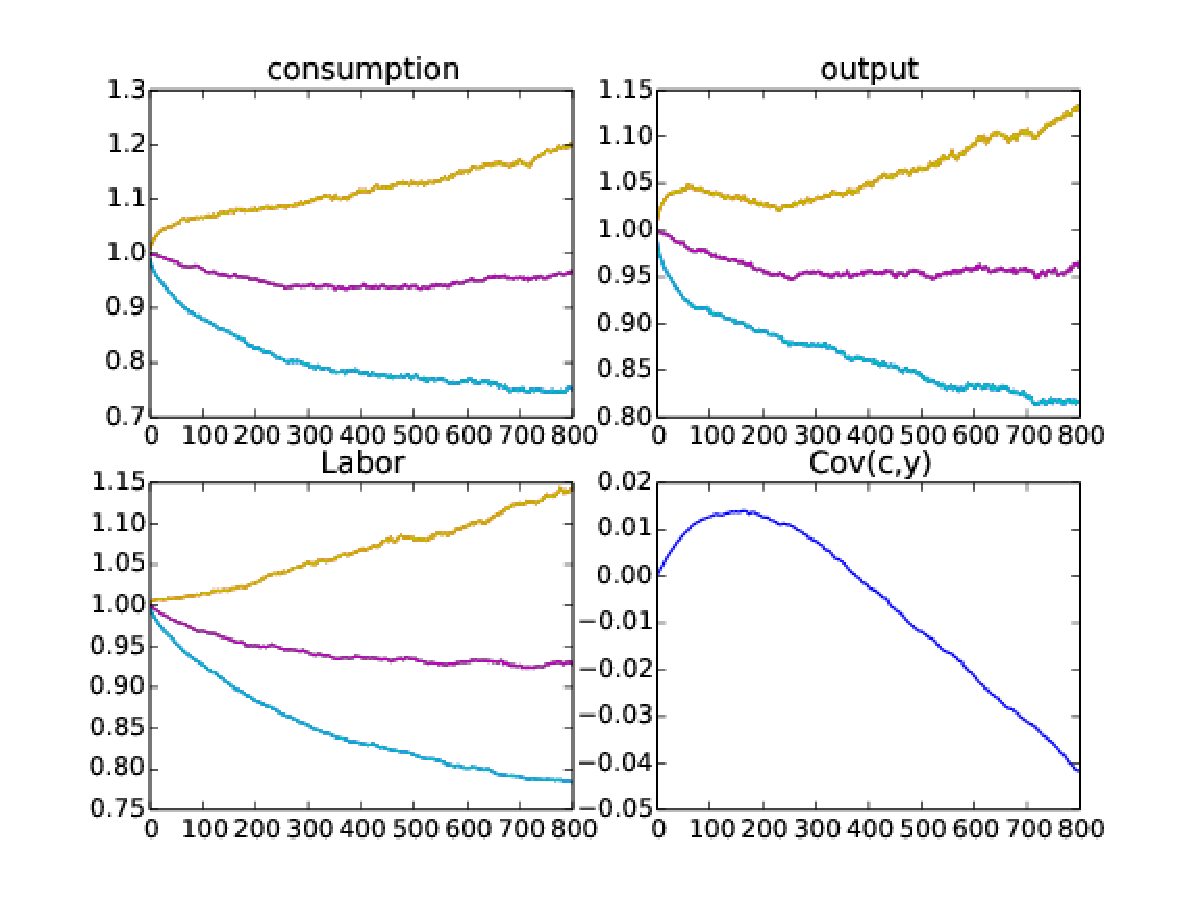
\includegraphics[width=0.8\textwidth]{Images/near_unit_quant.pdf}
 \caption{Inequality in the unit root  economy. The figure plots the quantiles for consumption, pre-tax labor earnings, labor and the covariance between consumption and pre-tax labor earnings}
 \label{fig:quant_pers}
 \end{figure}
\end{frame}


\begin{frame}
\frametitle {Tax rates in the close to unit root economy with aggregate shocks}

  \begin{figure}[htp]
 \centering
 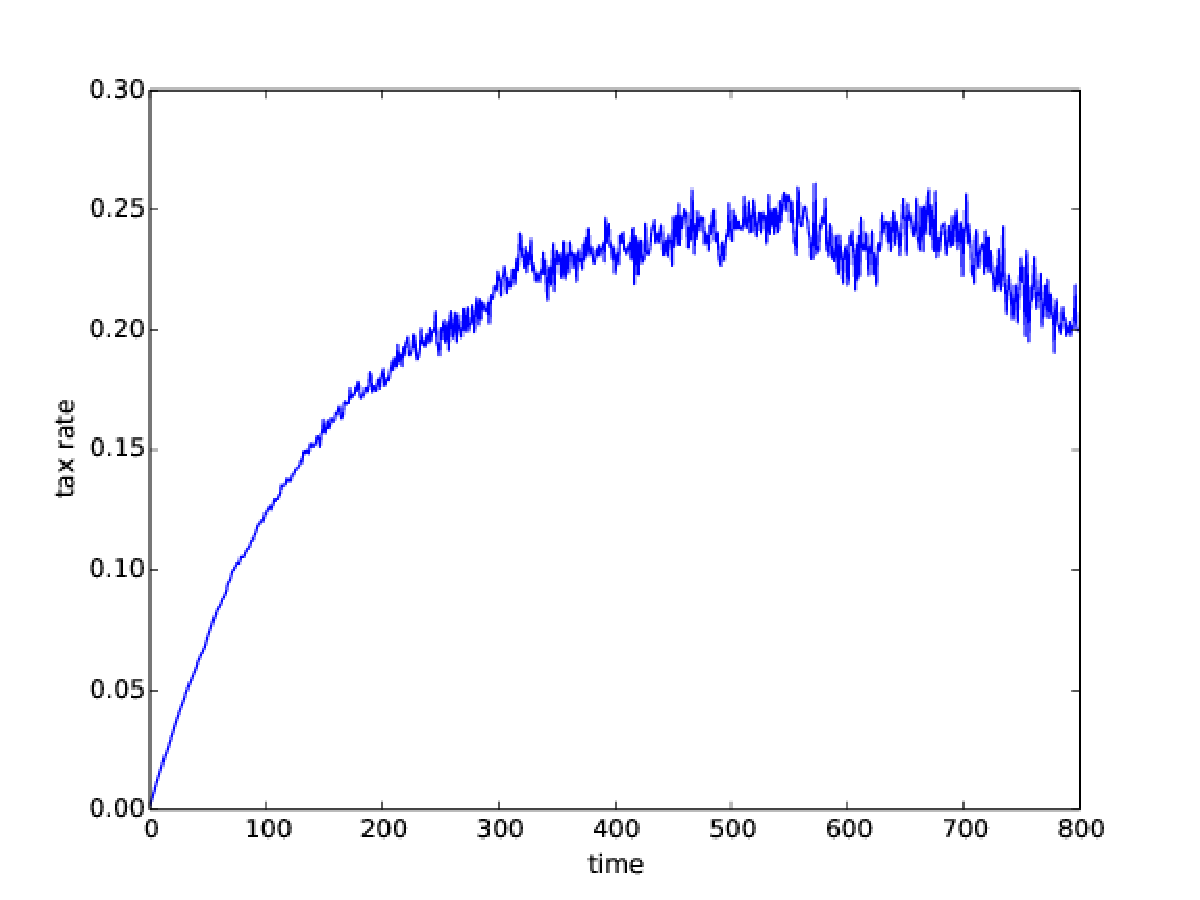
\includegraphics[width=0.9\textwidth]{Images/near_unit_agg.pdf}
 \caption{Taxes in the close to unit root economy with aggregate shocks }
 \label{fig:taxes_plots}
 \end{figure}
\end{frame}

\begin{frame}
 \frametitle{Calibrated Example}
Take a 2-shock 2-type economy with preferences $U(c,l)=\psi \log(c)+(1-\psi)\log(1-l)$ and with TFP shocks $\theta_i(s)$.

 \begin{itemize}

 \item Pick  baseline parameters to match some low frequency moments

 \item Calibrate outcome fluctuations to match three US recessions (i.e., 1991-92, 2001-02 and 2008-10):

 \begin{enumerate}
  \item The left tail of the cross-section distribution of labor income falls more than right tail
  \item Short term interest rates fall
  \item Booms last longer than recessions
 \end{enumerate}

 \end{itemize}

\end{frame}



\begin{frame}
 \frametitle{Calibration}

{\tiny
\begin{table}[htp]
{\tiny
\begin{tabular}{|l|l|l|c|}
\hline
Parameter & Value & Description &Target   \\ \hline
$\psi$ & 0.6994 &Frisch elasticity of labor supply & 0.5   \\
$\bar{\theta}_1 $ & 4& Log 90-10 wage ratio (Autor et al.) & 4   \\
$\bar{\theta}_2 $ & 1 &Normalize to 1 & 1  \\
$\beta$ & 0.98  &Average (annual) risk free interest rate & 2\%   \\
$\alpha_1$ & 0.69 & Marginal tax rate in the economy with no shocks & 20\% \\
$g$ & 12\%&Average pre-transfer expenditure- output ratio & 12 \% \\
$\frac{\hat {\theta}_2}{\hat {\theta}_1}$ & 2.5 & Relative drop in wage income of 10th
percentile & 2.5\\
$\hat{\theta}_1$ & 1.2\% & Average output loss& 3\% \\
$\hat{\beta}(s)$ & 1.96\%& Difference in real interest rates between booms and recession& 1.96\% \\
$P(r|r)$ & 0.63&Duration of recessions & 2.33 years \\
$P(b|b)$ & 0.84 &Duration of booms &7 years \\ \hline
\end{tabular}
}
\caption{Benchmark calibration}
\label{tab:Parameters}
\end{table}
}
Initial conditions chosen to make  debt to GDP ratio be 60\% \footnote{We use the same normalization as before i.e, the low productive agent has zero assets}
 \end{frame}

\begin{frame}
 \frametitle{Results: Some variants }
 We study perturbations of the Benchmark calibration
 \begin{enumerate}
\item Countercyclical interest rates
\item Acyclical interest rates by adjusting payoffs
\item A case with no inequality where all agents' productivities (TFP shock) fall in parallel
%\item \textbf{Government expenditure shocks}: A fall in $g$ that produces a comparable fall in output
\end{enumerate}

 \end{frame}
 


 \begin{frame}
  \frametitle{Short Run}
  To understand the short run responses
  \begin{itemize}
   %\item   Set the exogenous state $s_0$ to put as at the onset of a recession
   \item Solve the time 0 problem with identical initial conditions across
different settings. 
\item Use  optimal policies to compute fluctuations of
different components in the government budget constraint as we transition between booms to recessions
  \end{itemize}
 \end{frame}


 \begin{frame}
 \frametitle{Results: Short run}
 {\tiny
\begin{table}[tbp]
\begin{tabular}{|l|c|c|c|c|c|c|c|}
\hline
& \textbf{$\Delta g$} & \textbf{$\Delta B$} & \textbf{$\Delta T$} & \textbf{$%
\Delta [\tau\theta_1l_1]$} & \textbf{$\Delta [\tau\theta_2l_2]$} & \textbf{$%
\Delta Y$} & \textbf{$\Delta \tau$} \\ \hline
\textbf{Benchmark} & 0.0000 & -1.1561 & 0.6871 & -0.1593 & -0.3096 & -2.8536
& 0.3732 \\ \hline
\textbf{Acyclical Interest Rates} & 0.0000 & -1.1126 & 0.6591 & -0.1497 &
-0.3038 & -2.8613 & 0.3879 \\ \hline
\textbf{Countercyclical Interest Rates} & 0.0000 & -1.0794 & 0.6387 & -0.1415 &
-0.2992 & -2.8677 & 0.3997 \\ \hline
\textbf{No Inequality} & 0.0000 & -0.1380 &\color{red}{\textbf{ -0.5459}} & -0.5635 & -0.1204 &
-2.6294 & 0.0622 \\ \hline
%\textbf{Expenditure Shocks} & -7.5037 & 2.9137 & 2.8612 & -1.3759 & -0.3530 & -2.3443 &
%-1.1598 \\ \hline

\end{tabular}%

\caption{The tables summarizes the changes in the different components of the government budget as the economy transits from ``boom'' to  ``recession''.  All numbers except $\protect\tau $ are normalized by un-distorted GDP  and reported in percentages.
}

\label{tab:ShortRunPolicyResponses}
\end{table}
}
\begin{enumerate}
 \item For each variable
$z$ in the table we report  $\Delta z\equiv \left( z\left(
s_l|x_0,m_0,s_0\right) -z\left( s_h|x_0,m_0,s_0\right) \right) /\bar{Y}
$ where $\bar{Y}$ is average undistorted GDP in percentages
\item Predetermined variables like repayment on existing debt drop out
\begin{equation*}
\Delta [g]+\Delta[T]+ \Delta [B]=\Delta[\tau \theta_1 l_1]+ \Delta[\tau
\theta_2 l_2]
\end{equation*}%

\end{enumerate}

\small

 \end{frame}

\begin{frame}
 \frametitle{Conclusions}
 \begin{itemize}
  \item Concerns for redistribution imply costs of fluctuating transfers
  \item This affects the prescriptions of optimal policy for smoothing tax rates
  \item Market incompleteness is a key determinant of the invariant distribution of taxes and debt
  \item \textbf{Next step}: Calibrate a ``realistic'' idiosyncratic risk and aggregate risk process to learn about the quantitative implications of the model.

% \begin{itemize}
% \item Size of government debt alone is not informative $\Longrightarrow $
% need to know the net distribution of assets in the economy
%
% \item Ignoring heterogeneity produces misleading results about size and
% direction of the optimal policy response
%
% \item The better ability we have to tax assets, the less debt matters and
% can approximate complete markets closer
% \end{itemize}
 \end{itemize}

\end{frame}

\end{document}

\begin{frame}
\frametitle{Long Run: Steady States (SS)}
Let $\Psi \left( s;\bm{x},\bm{\rho },s\_\right) $ be an optimal  law of motion for the state variables
for the $t\geq1$ recursive problem, i.e.,


\[\Psi \left( s;\bm{x},%
\bm{\rho },s\_\right) =\left( x^{\prime }\left( s\right) ,\rho ^{\prime
}\left( s\right) \right) \]

attains $t\geq1$ value function given state $\left(\bm{x},\bm{\rho },s\_\right) $

\begin{definition}
 A steady state  $\left( \bm{x}^{SS},\bm{\rho} ^{SS}\right) $  satisfies $\left(\bm{ x}^{SS},\bm{\rho}
^{SS}\right) =\Psi \left( s;\bm{x}^{SS},\bm{\rho} ^{SS},s_{-}\right) $ for all $%
\,s,s\_$
\end{definition}
\vspace{3mm}
\emph{A steady state is a node at which the continuation allocation and tax schedule has no further history dependence. }
\end{frame}

\begin{frame}
\frametitle{Existence}
\begin{itemize}
 \item \textbf{Quasi-linear preferences:}
 \begin{enumerate}
                                           \item SS exists for a wide range of parameters and shocks
                                           \item The economy reaches a steady state in one period
                                           \item Output, tax rates are constant thereafter and levels are independent of initial conditions

\end{enumerate}
\emph{Dynamics of taxes are starkly different than AMSS}

 \item \textbf{General preferences:}
 \begin{enumerate}
 \item \emph{IID shocks with two values:} SS exists and continuation allocation is independent of initial conditions
 \item \emph{More general shocks:} There exists an ergodic region in which $\left( \bm{x},\bm{\rho} \right) $ is no longer constant, but  fluctuations are markedly reduced relative to the transient fluctuations that occur during an approach to  a SS
 \end{enumerate}
 \end{itemize}

\end{frame}


\begin{frame}
\frametitle{Intuition:  A two-agent example}

Consider I=2 with $\theta_1(s)>\theta_2=0$.

Two main forces determine the dynamics of the tax rate, transfers,  and assets:
\begin{itemize}
 \item \textbf{Fluctuations in inequality}  measured by spreads in marginal utilities
\item  \textbf{Fluctuations in interest rate}
\end{itemize}
For quasi linear preferences both forces are absent

\end{frame}

\begin{frame}
 \frametitle{3 Cases: Interest rates and relative assets}
 \begin{itemize}

 \item \textbf{Normalization:} By Ricardian equivalence, we can
 \begin{enumerate}
  \item Normalize $b_{2}(s)=0$
  \item Government assets:  $B(s)=-b_{1}(s)$
 \end{enumerate}
 \item \textbf{Interpretation:} The state variable $x\equiv U^2_c\tilde{b}_2=U^2_c[b_2-b_1]$. Under $b_{2}(s)=0$ normalization, $x$ is
 \begin{enumerate}
 \item Marginal utility scaled \textbf{debt} of the productive agent
 \item Marginal utility scaled \textbf{assets} held by the government
 \end{enumerate}
  \item \textbf{Results: }

\begin{tabular}{ l l c c }
 \emph{Interest rates} & \emph{Discount factors} &  $x=U^2_c[b_2-b_1]$\\
Countercyclical &$\beta(s_l)=\beta(s_h)$& $x>0$\\
Acyclical &$\beta(s_l)>\beta(s_h)$& $x>0$\\
Procyclical &$\beta(s_l)>>\beta(s_h)$& $x<0$\\
  \end{tabular}
  \end{itemize}

\end{frame}




\begin{frame}
\frametitle{ Inequality distortions}
Consider with case with acyclical interest rates

\vspace{2mm}
\MyArrow{} TFP: Adjust tax rate $\tau$ or transfers $T$, both are costly

\vspace{2mm}
Suppose $x=0$ (or $b_{2}(s)=b_{1}(s)$)
\begin{enumerate}
 \item Present value of earnings of productive agent are higher
 \item A reduction in transfers hurts the low productivity agent more
\end{enumerate}

Then

 \MyArrowUp{} $x$ is same as increasing the \textbf{debt} of the productive agent

\color{red} This drives the after-tax, after-interest incomes of both agents  closer
together



\end{frame}



% \begin{frame}
% \frametitle{ Inequality distortions}
%
% %\textcolor{blue}{Anmol XXXXX: may we please discuss this slide? It needs some clarification.}
% Start with a spread in discount factors set to equalize interest rates  across states,  i.e., $R(s_l)=R(s_h)$. Then SS  $x>0$
%
% \vspace{2mm}
% \MyArrow{} TFP ($\theta_1$): Adjust tax rate $\tau$ or transfers $T$, both are costly
%
% \vspace{2mm}
% Suppose $x=0$ or $b_{2}(s)=b_{1}(s)$,
%
% \MyArrow{} Then reductions in transfers hurt the low productivity agent more
%
% \vspace{2mm}
%
%  \emph{A fall in transfers that increases inequality gives rise to a cost  not present in  representative agent economies. This gives the planner an incentive to reduce the costs of  inequality distortions by $\ldots$ }
%
%  \MyArrowUp{} $x$
%
% \color{red} Reducing the relative asset holdings of the productive agent eventually drives the after-tax, after-interest incomes of both agents  closer
% together
%
%

%\end{frame}

\begin{frame}
\frametitle{Interest rate fluctuations}
\begin{itemize}

 \item \textbf{Countercyclical interest rates: }

 \MyArrow{} TFP: If the  tax rate  $\tau $ is left unchanged, the government faces a shortfall of revenues.

 \begin{enumerate}
 \item Reminder: $x$ is marginal utility scaled \textbf{assets} of the government
\item By holding positive assets the govt. can use higher interest income to offset some revenue losses from its tax on labor in recessions
  \item This force is present in representative agent economies with endogenous fluctuations in interest rates
\end{enumerate}

 \MyArrowUp{} $x$

 \item \textbf{Pro-cyclical interest rates:} If the interest rate is sufficiently low in a recession, the government may want to hold debt to free resources by lower interest payments.

 \MyArrow{} $x$
  \end{itemize}



\end{frame}
% \begin{frame}
%  \frametitle{Comparative statics with Pareto weights}
%    \begin{figure}[htp]
%  \centering
%  \includegraphics[width=\textwidth]{Draft25Graphs/SS_alpha1.eps}
%  \caption{Steady state govt. assets: $\tilde{b}_2(s)=\frac{\beta  x^{SS}}{U^2_c(s)}$ and taxes: $\tau^{SS}$ as a function of a (high skilled) agent 1's Pareto weight}
%  \label{fig: SS comparative}
%  \end{figure}
%
% \end{frame}

\begin{frame}
 \frametitle{Remarks on SS}
 \begin{itemize}
 \item Stability:
 \begin{enumerate}
  \item \textbf{Countercyclical interest rates:} Both forces push in the same direction $\rightarrow$ steady state is stable
  \item \textbf{Procyclical interest rates:} Both forces push in opposite direction $\rightarrow$ steady state is unstable
 \end{enumerate}
 \item For more than 2 agents, we have similar mechanics. In particular
  \begin{enumerate}
   \item Inequality distortions call for a negative correlation between productivities and (scaled) net assets
   \item Procyclical interest rates may flip the sign of the correlation between productivities and net assets to be positive.

   \begin{itemize}
   \item Low interest rates in recession prompts the government to hold debt
   \item By borrowing more from agents with higher productivities, the govt.\ can the reduce welfare costs of lowering transfer in adverse times
   \end{itemize}

  \end{enumerate}
\end{itemize}


\end{frame}

% \begin{frame}
% \frametitle{ case 1}
%
%
% Start with a spread in discount factors such that interest rates are equalized across i.e $R(s_l)=R(s_h)$. One can show that steady state $x>0$
%
% \begin{itemize}
%  \item The government can adjust two instruments in response  to an adverse  shock (i.e., a fall in $\theta_1$): it can either increase the  tax rate $\tau $ or it can decrease transfers $T.$ Both responses are distortionary
%  \item When agents' asset holdings are identical, a decrease in transfers  disproportionately
% affects a low-skilled agent, so his marginal utility falls by more than does the marginal utility of a high-skilled agent.
% \item  Consequently, a
% decrease in transfers increases inequality, giving rise to a cost  not present in  representative agent economies.
% \item  The government can reduce the costs of  inequality distortions by choosing tax rate policies that make the net asset positions of  the high-skilled agent
% decrease over time.
% \item this makes the two agents' after-tax and after-interest income  become closer, allowing decreases in transfers to have smaller effects on inequality in
% marginal utilities.
%  \end{itemize}
%
% \end{frame}

\begin{frame}
 \frametitle{Numerical Example}

 Use a  calibrated version of the economy to
 \begin{itemize}
  \item Approximate magnitudes of these forces and
  \item Study optimal policy responses at business cycle frequencies when an economy is possibly far away from a steady state
 \end{itemize}
 \end{frame}
 \begin{frame}
 \frametitle{Numerical Example: Calibration}
Take a 2-shock 2-type economy with preferences $U(c,l)=\psi \log(c)+(1-\psi)\log(1-l)$ and allow $\theta_i(s),\beta(s),g(s)$ to depend on $s$.

 \begin{itemize}

 \item Pick  baseline parameters to match some low frequency moments

 \item Calibrate outcome fluctuations to match three US recessions (i.e., 1991-92, 2001-02 and 2008-10):

 \begin{enumerate}
  \item The left tail of the cross-section distribution of labor income falls more than right tail
  \item Short term interest rates fall
  \item Booms last longer than recessions
 \end{enumerate}

 \end{itemize}

\end{frame}



\begin{frame}
 \frametitle{Calibration}

{\tiny
\begin{table}[htp]
{\tiny
\begin{tabular}{|l|l|l|c|}
\hline
Parameter & Value & Description &Target   \\ \hline
$\psi$ & 0.6994 &Frisch elasticity of labor supply & 0.5   \\
$\bar{\theta}_1 $ & 4& Log 90-10 wage ratio (Autor et al.) & 4   \\
$\bar{\theta}_2 $ & 1 &Normalize to 1 & 1  \\
$\beta$ & 0.98  &Average (annual) risk free interest rate & 2\%   \\
$\alpha_1$ & 0.69 & Marginal tax rate in the economy with no shocks & 20\% \\
$g$ & 12\%&Average pre-transfer expenditure- output ratio & 12 \% \\
$\frac{\hat {\theta}_2}{\hat {\theta}_1}$ & 2.5 & Relative drop in wage income of 10th
percentile & 2.5\\
$\hat{\theta}_1$ & 1.2\% & Average output loss& 3\% \\
$\hat{\beta}(s)$ & 1.96\%& Difference in real interest rates between booms and recession& 1.96\% \\
$P(r|r)$ & 0.63&Duration of recessions & 2.33 years \\
$P(b|b)$ & 0.84 &Duration of booms &7 years \\ \hline
\end{tabular}
}
\caption{Benchmark calibration}
\label{tab:Parameters}
\end{table}
}
Initial conditions chosen to make  debt to GDP ratio be 60\% \footnote{We use the same normalization as before i.e, the low productive agent has zero assets}
 \end{frame}

\begin{frame}
 \frametitle{Results: Some variants }
 We study perturbations of the Benchmark calibration
 \begin{enumerate}
\item \textbf{Acyclical interest rates}: Smaller spread in discount factor shocks
\item \textbf{Countercyclical interest rates}: No discount factor shocks
\item \textbf{No inequality}: Equal fall in all agents' productivities (TFP shock) and no discount factor shocks
%\item \textbf{Government expenditure shocks}: A fall in $g$ that produces a comparable fall in output
\end{enumerate}

 \end{frame}


\begin{frame}
 \frametitle{Results: Long run}

  \begin{figure}[htp]
 \centering
 \includegraphics[width=\textwidth]{Draft25Graphs/LongSimulationsColor.eps}
 \caption{Govt. debt for several economies: benchmark (o), acyclical interest rates (\color{blue}+\color{black}), countercyclical interest rates (\color{red}$\diamond$\color{black}) and no inequality shocks \scriptsize (\color{green}$\square$\color{green}\normalsize) }
 %\caption{ Debt benchmark $\circle$, acyclical interest rates + , countercyclical interest rates $\diamond$ }% and no inequality shocks {\scriptsize $\square$ \normalsize}}
 \label{fig:LongSimulations}
 \end{figure}


 \end{frame}

 \begin{frame}[label=main]
  \frametitle{Observations}
  \begin{itemize}
   \item Long run tendency to converge to some ergodic set. But convergence is very slow
   \hyperlink{convergence}{\beamerbutton{more details on speed of convergence}}.
   \item With low discount factor shocks, outcomes approach positive govt. assets
   \item With high discount factor shocks that produce procyclical real interest rates, there is no tendency to reduce govt. debt even after 5000 years
  \end{itemize}

 \end{frame}

 \begin{frame}
  \frametitle{Short Run}
  To understand the short run responses
  \begin{itemize}
   %\item   Set the exogenous state $s_0$ to put as at the onset of a recession
   \item Solve the time 0 problem with identical initial conditions across
different settings. This pins down the initial state vector  $x_0,\rho_0$  that appears in our time $0$ Bellman equation
\item Use  optimal policies to compute fluctuations of
different components in the government budget constraint as we transition between booms to recessions
  \end{itemize}
 \end{frame}


 \begin{frame}
 \frametitle{Results: Short run}
 {\tiny
\begin{table}[tbp]
\begin{tabular}{|l|c|c|c|c|c|c|c|}
\hline
& \textbf{$\Delta g$} & \textbf{$\Delta B$} & \textbf{$\Delta T$} & \textbf{$%
\Delta [\tau\theta_1l_1]$} & \textbf{$\Delta [\tau\theta_2l_2]$} & \textbf{$%
\Delta Y$} & \textbf{$\Delta \tau$} \\ \hline
\textbf{Benchmark} & 0.0000 & -1.1561 & 0.6871 & -0.1593 & -0.3096 & -2.8536
& 0.3732 \\ \hline
\textbf{Acyclical Interest Rates} & 0.0000 & -1.1126 & 0.6591 & -0.1497 &
-0.3038 & -2.8613 & 0.3879 \\ \hline
\textbf{Countercyclical Interest Rates} & 0.0000 & -1.0794 & 0.6387 & -0.1415 &
-0.2992 & -2.8677 & 0.3997 \\ \hline
\textbf{No Inequality} & 0.0000 & -0.1380 &\color{red}{\textbf{ -0.5459}} & -0.5635 & -0.1204 &
-2.6294 & 0.0622 \\ \hline
%\textbf{Expenditure Shocks} & -7.5037 & 2.9137 & 2.8612 & -1.3759 & -0.3530 & -2.3443 &
%-1.1598 \\ \hline

\end{tabular}%

\caption{The tables summarizes the changes in the different components of the government budget as the economy transits from ``boom'' to  ``recession''.  All numbers except $\protect\tau $ are normalized by un-distorted GDP  and reported in percentages.
}

\label{tab:ShortRunPolicyResponses}
\end{table}
}
\begin{enumerate}
 \item For each variable
$z$ in the table we report  $\Delta z\equiv \left( z\left(
s_l|x_0,\rho_0,s_0\right) -z\left( s_h|x_0,\rho_0,s_0\right) \right) /\bar{Y}
$ where $\bar{Y}$ is average undistorted GDP in percentages
\item Predetermined variables like repayment on existing debt drop out
\begin{equation*}
\Delta [g]+\Delta[T]+ \Delta [B]=\Delta[\tau \theta_1 l_1]+ \Delta[\tau
\theta_2 l_2]
\end{equation*}%

\end{enumerate}

\small

 \end{frame}

\begin{frame}
 \frametitle{Conclusions}
\begin{itemize}
\item Size of government debt alone is irrelevant $\Longrightarrow $
need to know the  distribution of net assets
\item Optimal tax and transfer scheme balance
\begin{enumerate}
 \item welfare losses from fluctuating taxes
 \item welfare losses from fluctuating transfers
\end{enumerate}
%\item Since welfare costs depend on the how debt is distributed, the planner has incentives to move  net assets over time
\item With incomplete markets, interest rate fluctuations are a  key determinant of  long-run correlations between productivities and net assets
\item Ignoring heterogeneity produces misleading results about the size and direction of short run optimal policy responses
\end{itemize}

\end{frame}
\appendix
\section{More}

\begin{frame}[label=convergence]
\frametitle{Speed of convergence  (I) }
Suppose we are in the binary-IID world where steady states are deterministic.


\begin{itemize}
\item The optimal policy induces two \emph{risk adjusted} martingales
\begin{enumerate}
\item Multiplier on the implementability constraint : $\bm{\mu}_{t}$
\item The ratio of marginal utilities: $\bm{\rho}_{t}$
\end{enumerate}
 \item One can represent the optimal allocation recursively in terms of $\{\bm \mu(s^{t-1}),\bm \rho(s^{t-1})\}$ and $s_t$.
\item Why $(\bm{\mu},\bm{\rho})$ instead of $(\bm{x},\bm{\rho})$?
\item Linearize optimal policies for each $s_t$ around the constant steady state.
\item Study the eigenvalues of the conditional mean and variance dynamics (these are deterministic linear systems)
\end{itemize}

\end{frame}


\begin{frame}
\frametitle{Speed of convergence  (II) }
Let $\hat{\Psi}_{t}= \left[\bmat \bm{\mu}_{t} - \bm{\mu}^{SS}\\ \bm \rho_t - \bm \rho^{SS}\emat\right]$. Then
\begin{equation*}
 \hat{\Psi}_{t+1}=B(s_{t+1})\hat{\Psi}_t
\end{equation*}
This linearized system has coefficients that are functions of the shock $s$.
\small

\begin{proposition}\label{prop: localstability}
If the (real part) of eigenvalues of $\mathbb{E}B(s)$ are less than 1,  the system  converges to zero  in mean. Further for large $t$, the conditional variance of $\hat{\Psi}$, denoted by $\Sigma_{\Psi,t}$, follows a deterministic process governed by
\[\text{vec}(\Sigma_{\Psi,t})=\hat{B} \text{vec}(\Sigma_{\Psi,t-1}),\]	
where $\hat{B}$ is a square matrix of dimension $(2N-2)^2$. In addition,  if the (real parts) of eigenvalues of $\hat{B}$ are all less than 1, the system converges in probability.
\end{proposition}

\color{red}\emph{The eigenvalues (in particular the largest one) are instructive not only for whether the system is locally stable but also for how quickly the steady state is reached}

\end{frame}

\begin{frame}
\frametitle{Speed of convergence: Size of shocks and risk aversion}

  \begin{figure}[htp]
  \tiny
 \centering
 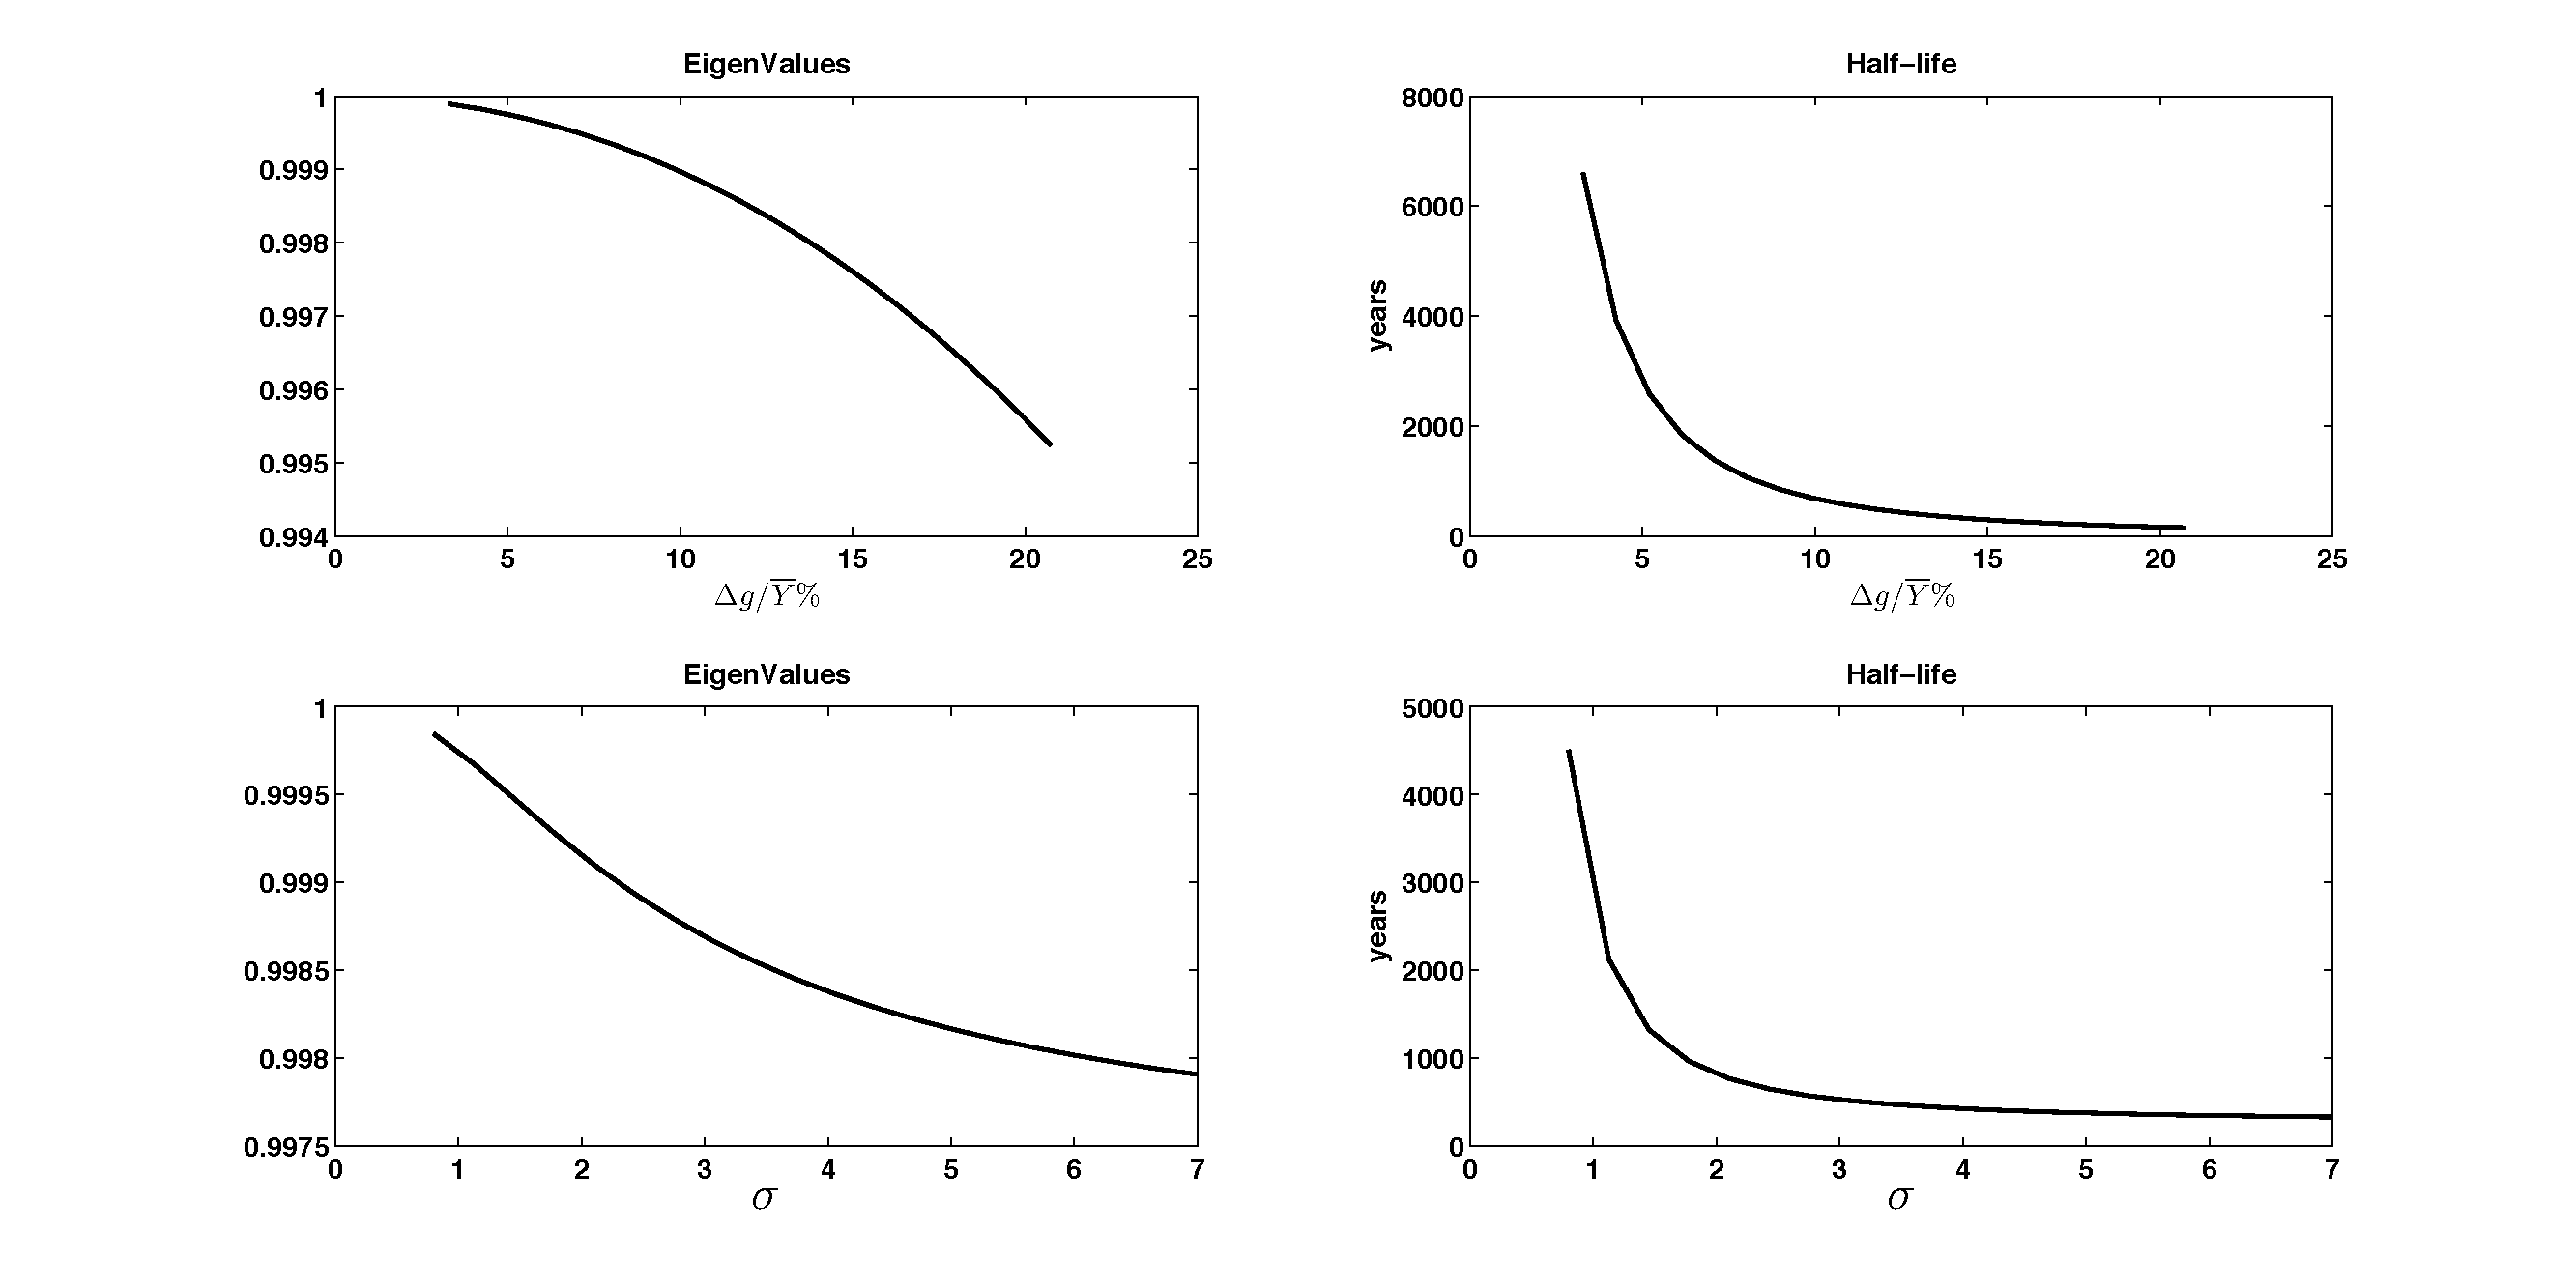
\includegraphics[width=\textwidth]{Draft25Graphs/eigenvalues.eps}
 \caption{\tiny{The top (bottom) panel plots the dominant eigenvalue of $\hat{B}$ and the associated half life as we increase
the spread between the expenditure levels (risk aversion).}}
 \label{fig: Eigenvalues}
 \end{figure}
 Back to \hyperlink{main}{\beamerbutton{main}}
 \end{frame}
 \end{document}

%
% \begin{itemize}
% \item Size of government debt alone is not informative $\Longrightarrow $
% need to know the net distribution of assets in the economy
%
% \item Ignoring heterogeneity produces misleading results about size and
% direction of the optimal policy response
%
% \item The better ability we have to tax assets, the less debt matters and
% can approximate complete markets closer
% \end{itemize}
%
% %TCIMACRO{\TeXButton{EndFrame}{\end{frame}}}%
% %BeginExpansion
% \end{frame}%
% %EndExpansion
%
% \end{document}
